%% ma: L12-B01-0016
%% lop: 12
%% chuong: 1
%% bai: 1
%% dang: 12.1.11
%% loai: TN4
%% muc: NB
%% dap_an: "D"
%% nguon: "Ảnh giáo viên gửi 11/10/2026 (Đề kiểm tra giữa HK1 Toán 12, THPT Việt Đức 2026-2027, mã đề 0103), Phần I Câu 8"
%% kien_thuc: "Bài 1 (đọc điểm cực đại của đồ thị từ bảng biến thiên)"
%% trang_thai: cho-duyet
%% ly_do: "Dạng mới đề xuất, chờ giáo viên duyệt."
\begin{ex}
Cho hàm số $y=f(x)$ liên tục trên $\mathbb R$ và có bảng biến thiên sau:
\begin{center}
\begin{tikzpicture}
  \tkzTabInit[lgt=1.4,espcl=3.2]{$x$/.8,$f'(x)$/.8,$f(x)$/2.2}{$-\infty$,$-2$,$1$,$+\infty$}
  \tkzTabLine{,+,0,-,0,+,}
  \tkzTabVar{-/$-\infty$,+/$4$,-/$-1$,+/$+\infty$}
\end{tikzpicture}
\end{center}
Điểm cực đại của đồ thị hàm số là
\choice{$(1;-1)$}{$(-2;-1)$}{$(1;4)$}{\True $(-2;4)$}
\loigiai{Từ bảng biến thiên, $f'(x)$ đổi dấu từ $+$ sang $-$ khi qua $x=-2$ và $f(-2)=4$. Vậy điểm cực đại của đồ thị hàm số là $(-2;4)$.}
\end{ex}
